
\documentclass[letterpaper,hide notes,xcolor={table,svgnames},pdftex]{beamer}
\def\showexamples{t}


%\usepackage[svgnames]{xcolor}

%% Demo talk
%\documentclass[letterpaper,notes=show]{beamer}

\usecolortheme{crane}
\setbeamertemplate{navigation symbols}{}

\usetheme{MyPittsburgh}
%\usetheme{Frankfurt}

%\usepackage{tipa}

\usepackage{hyperref}
\usepackage{graphicx,xspace}
\usepackage[normalem]{ulem}

\newcommand\SF[1]{$\bigstar$\footnote{SF: #1}}



\newcounter{tmpnumSlide}
\newcounter{tmpnumNote}

% old question code
%\newcommand\question[1]{{$\bigstar$ \small \onlySlide{2}{#1}}}
% \newcommand\nquestion[1]{\ifdefined \presentationonly \textcircled{?} \fi \note{\par{\Large \textbf{?}} #1}}
% \newcommand\nanswer[1]{\note{\par{\Large \textbf{A}} #1}}


 \newcommand\mnote[1]{%
   \addtocounter{tmpnumSlide}{1}
   \ifdefined\showcues {~\tiny\fbox{\arabic{tmpnumSlide}}}\fi
   \note{\setlength{\parskip}{1ex}\addtocounter{tmpnumNote}{1}\textbf{\Large \arabic{tmpnumNote}:} {#1\par}}}

\newcommand\mmnote[1]{\note{\setlength{\parskip}{1ex}#1\par}}

%\newcommand\mnote[2][]{\ifdefined\handoutwithnotes {~\tiny\fbox{#1}}\fi
% \note{\setlength{\parskip}{1ex}\textbf{\Large #1:} #2\par}}

%\newcommand\mnote[2][]{{\tiny\fbox{#1}} \note{\setlength{\parskip}{1ex}\textbf{\Large #1:} #2\par}}

\newcommand\mquestion[2]{{~\color{red}\fbox{?}}\note{\setlength{\parskip}{1ex}\par{\Large \textbf{?}} #1} \note{\setlength{\parskip}{1ex}\par{\Large \textbf{A}} #2\par}\ifdefined \presentationonly \pause \fi}

\newcommand\blackboard[1]{%
\ifdefined   \showblackboard
  {#1}
  \else {\begin{center} \fbox{\colorbox{blue!30}{%
         \begin{minipage}{.95\linewidth}%
           \hspace{\stretch{1}} Some space intentionally left blank; done at the blackboard.%
         \end{minipage}}}\end{center}}%
         \fi%
}



%\newcommand\q{\tikz \node[thick,color=black,shape=circle]{?};}
%\newcommand\q{\ifdefined \presentationonly \textcircled{?} \fi}

\usepackage{listings}
\lstset{%
  keywordstyle=\bfseries,
  aboveskip=15pt,
  belowskip=15pt,
  captionpos=b,
  identifierstyle=\ttfamily,
  escapeinside={(*@}{@*)},
  stringstyle=\ttfamiliy,
  frame=lines,
  numbers=left, basicstyle=\scriptsize, numberstyle=\tiny, stepnumber=0, numbersep=2pt}

\usepackage{siunitx}
\newcommand\sius[1]{\num[group-separator = {,}]{#1}\si{\micro\second}}
\newcommand\sims[1]{\num[group-separator = {,}]{#1}\si{\milli\second}}
\newcommand\sins[1]{\num[group-separator = {,}]{#1}\si{\nano\second}}
\sisetup{group-separator = {,}, group-digits = true}

%% -------------------- tikz --------------------
\usepackage{tikz}
\usetikzlibrary{positioning}
\usetikzlibrary{arrows,backgrounds,automata,decorations.shapes,decorations.pathmorphing,decorations.markings,decorations.text}

\tikzstyle{place}=[circle,draw=blue!50,fill=blue!20,thick, inner sep=0pt,minimum size=6mm]
\tikzstyle{transition}=[rectangle,draw=black!50,fill=black!20,thick, inner sep=0pt,minimum size=4mm]

\tikzstyle{block}=[rectangle,draw=black, thick, inner sep=5pt]
\tikzstyle{bullet}=[circle,draw=black, fill=black, thin, inner sep=2pt]

\tikzstyle{pre}=[<-,shorten <=1pt,>=stealth',semithick]
\tikzstyle{post}=[->,shorten >=1pt,>=stealth',semithick]
\tikzstyle{bi}=[<->,shorten >=1pt,shorten <=1pt, >=stealth',semithick]

\tikzstyle{mut}=[-,>=stealth',semithick]

\tikzstyle{treereset}=[dashed,->, shorten >=1pt,>=stealth',thin]

\usepackage{ifmtarg}
\usepackage{xifthen}
\makeatletter
% new counter to now which frame it is within the sequence
\newcounter{multiframecounter}
% initialize buffer for previously used frame title
\gdef\lastframetitle{\textit{undefined}}
% new environment for a multi-frame
\newenvironment{multiframe}[1][]{%
\ifthenelse{\isempty{#1}}{%
% if no frame title was set via optional parameter,
% only increase sequence counter by 1
\addtocounter{multiframecounter}{1}%
}{%
% new frame title has been provided, thus
% reset sequence counter to 1 and buffer frame title for later use
\setcounter{multiframecounter}{1}%
\gdef\lastframetitle{#1}%
}%
% start conventional frame environment and
% automatically set frame title followed by sequence counter
\begin{frame}%
\frametitle{\lastframetitle~{\normalfont(\arabic{multiframecounter})}}%
}{%
\end{frame}%
}
\makeatother

\makeatletter
\newdimen\tu@tmpa%
\newdimen\ydiffl%
\newdimen\xdiffl%
\newcommand\ydiff[2]{%
    \coordinate (tmpnamea) at (#1);%
    \coordinate (tmpnameb) at (#2);%
    \pgfextracty{\tu@tmpa}{\pgfpointanchor{tmpnamea}{center}}%
    \pgfextracty{\ydiffl}{\pgfpointanchor{tmpnameb}{center}}%
    \advance\ydiffl by -\tu@tmpa%
}
\newcommand\xdiff[2]{%
    \coordinate (tmpnamea) at (#1);%
    \coordinate (tmpnameb) at (#2);%
    \pgfextractx{\tu@tmpa}{\pgfpointanchor{tmpnamea}{center}}%
    \pgfextractx{\xdiffl}{\pgfpointanchor{tmpnameb}{center}}%
    \advance\xdiffl by -\tu@tmpa%
}
\makeatother
\newcommand{\copyrightbox}[3][r]{%
\begin{tikzpicture}%
\node[inner sep=0pt,minimum size=2em](ciimage){#2};
\usefont{OT1}{phv}{n}{n}\fontsize{4}{4}\selectfont
\ydiff{ciimage.south}{ciimage.north}
\xdiff{ciimage.west}{ciimage.east}
\ifthenelse{\equal{#1}{r}}{%
\node[inner sep=0pt,right=1ex of ciimage.south east,anchor=north west,rotate=90]%
{\raggedleft\color{black!50}\parbox{\the\ydiffl}{\raggedright{}#3}};%
}{%
\ifthenelse{\equal{#1}{l}}{%
\node[inner sep=0pt,right=1ex of ciimage.south west,anchor=south west,rotate=90]%
{\raggedleft\color{black!50}\parbox{\the\ydiffl}{\raggedright{}#3}};%
}{%
\node[inner sep=0pt,below=1ex of ciimage.south west,anchor=north west]%
{\raggedleft\color{black!50}\parbox{\the\xdiffl}{\raggedright{}#3}};%
}
}
\end{tikzpicture}
}


%% --------------------

%\usepackage[excludeor]{everyhook}
%\PushPreHook{par}{\setbox0=\lastbox\llap{MUH}}\box0}

%\vspace*{\stretch{1}

%\setbox0=\lastbox \llap{\textbullet\enskip}\box0}

\setlength{\parskip}{\fill}

\newcommand\noskips{\setlength{\parskip}{1ex}}
\newcommand\doskips{\setlength{\parskip}{\fill}}

\newcommand\xx{\par\vspace*{\stretch{1}}\par}
\newcommand\xxs{\par\vspace*{2ex}\par}
\newcommand\tuple[1]{\langle #1 \rangle}
\newcommand\code[1]{{\sf \footnotesize #1}}
\newcommand\ex[1]{\uline{Example:} \ifdefined \presentationonly \pause \fi
  \ifdefined\showexamples#1\xspace\else{\uline{\hspace*{2cm}}}\fi}

\newcommand\ceil[1]{\lceil #1 \rceil}


\AtBeginSection[]
{
   \begin{frame}
       \frametitle{Outline}
       \tableofcontents[currentsection]
   \end{frame}
}



\pgfdeclarelayer{edgelayer}
\pgfdeclarelayer{nodelayer}
\pgfsetlayers{edgelayer,nodelayer,main}

\tikzstyle{none}=[inner sep=0pt]
\tikzstyle{rn}=[circle,fill=Red,draw=Black,line width=0.8 pt]
\tikzstyle{gn}=[circle,fill=Lime,draw=Black,line width=0.8 pt]
\tikzstyle{yn}=[circle,fill=Yellow,draw=Black,line width=0.8 pt]
\tikzstyle{empty}=[circle,fill=White,draw=Black]
\tikzstyle{bw} = [rectangle, draw, fill=blue!20, 
    text width=4em, text centered, rounded corners, minimum height=2em]
    
    \newcommand{\CcNote}[1]{% longname
	This work is licensed under the \textit{Creative Commons #1 3.0 License}.%
}
\newcommand{\CcImageBy}[1]{%
	\includegraphics[scale=#1]{creative_commons/cc_by_30.pdf}%
}
\newcommand{\CcImageSa}[1]{%
	\includegraphics[scale=#1]{creative_commons/cc_sa_30.pdf}%
}
\newcommand{\CcImageNc}[1]{%
	\includegraphics[scale=#1]{creative_commons/cc_nc_30.pdf}%
}
\newcommand{\CcGroupBySa}[2]{% zoom, gap
	\CcImageBy{#1}\hspace*{#2}\CcImageNc{#1}\hspace*{#2}\CcImageSa{#1}%
}
\newcommand{\CcLongnameByNcSa}{Attribution-NonCommercial-ShareAlike}

\newenvironment{changemargin}[1]{% 
  \begin{list}{}{% 
    \setlength{\topsep}{0pt}% 
    \setlength{\leftmargin}{#1}% 
    \setlength{\rightmargin}{1em}
    \setlength{\listparindent}{\parindent}% 
    \setlength{\itemindent}{\parindent}% 
    \setlength{\parsep}{\parskip}% 
  }% 
  \item[]}{\end{list}} 



\usepackage{tikz-3dplot}
\DeclareUrlCommand\j{}


\title{Lecture 29 --- Software Statistics}

\author{Eric David Hollbach \& Mahesh Tripunitara \\ \small \texttt{edhollbach@uwaterloo.ca} \& \texttt{tripunit@uwaterloo.ca}}
\institute{Department of Electrical and Computer Engineering \\
  University of Waterloo}
\date{\today}

\begin{document}

\begin{frame}
  \titlepage
\end{frame}

\begin{frame}
\frametitle{The Setting}
\begin{changemargin}{1cm}

The Java SDK specifies an interface called \j{Set}. 

Its semantics is the mathematical notion of a set --- an unordered collection of unique items.

Several implementations of \j{Set} are provided by the SDK. 

Are they all the same? 

If not, which one should we use?

\end{changemargin}
\end{frame}

\begin{frame}
\frametitle{The Setting}
\begin{changemargin}{1cm}

They are not identical, so we expect that the answer is: ``it depends on your application.''

We need comparison criteria.

We want these two operations to be fast:
\begin{enumerate}
    \item Addition; and
    \item Membership-checking;
\end{enumerate}

\end{changemargin}
\end{frame}


\begin{frame}
\frametitle{The Setting}
\begin{changemargin}{1cm}

These criteria, in turn, provide an objective way of evaluating if
one implementation is better than another. 

The goal is more modest than the absolute criterion of ``fast''. 

We are just figuring out if one set-implementation
is ``better than'' (faster than) another in these two operations.

\end{changemargin}
\end{frame}

\begin{frame}
\frametitle{Evaluating Implementations}
\begin{changemargin}{1cm}

The question now is: how can we evaluate two given implementations in a rigorous and consistent way?

Statistics!

\end{changemargin}
\end{frame}

\begin{frame}
\frametitle{Alice's Process}
\begin{changemargin}{1cm}

\begin{enumerate}
\item Randomly choose a bunch of integers (let's say 100).

\item Use some API for measuring time on the computer.
Write Java code to measure the time it takes to add each of
those integers to an instance of a set-implementation $I_1$,
starting at $I_1 = \emptyset$ (the empty set). Compute the average time, $a_1$.

\item Repeat for an instance of another set-implementation
$I_2$ to get the average $a_2$ for it.

\item If $a_1 < a_2$, conclude that the first set-implementation
is better than the second from the standpoint of additions to the set.
\end{enumerate}

\end{changemargin}
\end{frame}

\begin{frame}
\frametitle{Problems with the Above}
\begin{changemargin}{1cm}

\begin{itemize}
    \item How do we know that the random set of integers Alice chooses
	is representative?
    \item Do we have to consider the order in which we add
	the integers?
    \item Why is it meaningful to use the average to draw our
	conclusion?
    \item How do we know that the averages are \emph{statistically
	significant}? 
    \item Computers demonstrate considerable variations over
	time in how long they take to perform an operation.
\end{itemize}

\end{changemargin}
\end{frame}

\begin{frame}
\frametitle{Addressing the Problems}
\begin{changemargin}{1cm}

Ideally, we will have good answers to all of the above questions.

Even if we are unable to conclusively address a concern such
as the above, it is very important to recognize the concern. 

And
at the minimum articulate an assumption explicitly.

\end{changemargin}
\end{frame}

\begin{frame}
\frametitle{Statistics Basics}
\begin{changemargin}{1cm}

A (mathematical) \emph{function} is defined as follows. 

Given two sets, a domain and a range, a function associates a member of the
range with every member of the domain.

We can associate the time it takes to add or membership-check
an element against a set as a \emph{random variable}.

\end{changemargin}
\end{frame}

\begin{frame}
\frametitle{Random Variables}
\begin{changemargin}{1cm}

A random variable is a function
$f\!\! : E \longrightarrow \mathbb{R}$\\
\quad $E$ is a set of \emph{events}, and\\
\quad $\mathbb{R}$ is the set of real numbers.


The range is the time it takes to add a member or check membership.

In this example, $E$ is the set of all integers.

\end{changemargin}
\end{frame}


\begin{frame}
\frametitle{Random Variables}
\begin{changemargin}{1cm}

we adopt two random variables, $a$ (adding) and $m$(membership-checking). 

Each maps an integer to a time-value. 

We associate a random variable with a \emph{probability distribution}.

\end{changemargin}
\end{frame}


\begin{frame}
\frametitle{Probability Distribution}
\begin{changemargin}{1cm}

A probability distribution is itself a function. 
It maps
each event in $E$ to a probability that it occurs.

For example, it is possible that the
probability that we add the integer $15$ to a set,
is different from the probability that we add $32$.

Thus, the probability we associate with the event
$\tuple{15}$ is different from the probability
we associate with the event $\tuple{32}$.

\end{changemargin}
\end{frame}


\begin{frame}
\frametitle{Using our Random Variables}
\begin{changemargin}{1cm}

If we can discover this $a(e)$ and $m(e)$
for a ``typical'' $e \in E$ for
two different set-implementations, then we can draw a conclusion.


This has two challenges: \\
\quad what is a ``typical'' $e \in E$; and\\
\quad how do we compute $a$ and $m$ even if we know this $e$?

\end{changemargin}
\end{frame}


\begin{frame}
\frametitle{Characterizing $a$ and $m$}
\begin{changemargin}{1cm}

The domain of a random variable ($E$, above) is called a
\emph{population}. 

To characterize a random variable, an approach
is to determine to what value in the range it maps every member of
the population, and then compute a \emph{central tendency} or
\emph{centre} of those values.

\end{changemargin}
\end{frame}


\begin{frame}
\frametitle{The Centre}
\begin{changemargin}{1cm}

A centre, as its name suggests, represents the ``middle'' of
all possible values. 

The \emph{average}, the sum of all values
divided by the number of values, is a centre. 

Other examples of
centres are the \emph{median} and \emph{trimean}.

\end{changemargin}
\end{frame}


\begin{frame}
\frametitle{Choice of a Centre}
\begin{changemargin}{1cm}

The choice of a centre is crucial. 

Not every centre is
\emph{robust} to \emph{outliers}. 

An outlier is a value
that occurs infrequently. 

Robustness is the property that
a centre is representative of the ``middle'' notwithstanding
the presence of outliers. 

\end{changemargin}
\end{frame}


\begin{frame}
\frametitle{Sampling}
\begin{changemargin}{1cm}
It is often impractical or even impossible to compute a
centre for the entire population. 

If the population
is all Canadians, determining the value of a random variable
for every Canadian may be deemed too expensive.

Consequently, we collect data \emph{samples}.

The procedure by which we collect samples is important.

Otherwise,
the samples may not reflect the properties of the population.

\end{changemargin}
\end{frame}


\begin{frame}
\frametitle{Sampling}
\begin{changemargin}{1cm}

Given a random variable $X$ whose underlying
probability distribution is $P$, a well-accepted property of
samples is that they are: 
\begin{enumerate}
\item \emph{independent and identically
distributed} (iid); and
\item each sample, when viewed as a
random variable
in its own right, has the same distribution $P$ as $X$.
\end{enumerate}

\end{changemargin}
\end{frame}


\begin{frame}
\frametitle{Sampling Example}
\begin{changemargin}{1cm}

Suppose $X$ is the random variable that is the height
of a person. 
The manner in which we collect samples must
reflect the distribution of heights amongst individuals.

If the probability that there exists a person of height $h$ in
the entire population is $\rho$, then the probability that height
$h$ ends up in our set of samples must be $\rho$.

\end{changemargin}
\end{frame}

\begin{frame}
\frametitle{How To Sample}
\begin{changemargin}{1cm}

There are three issues to resolve in sampling:

\begin{enumerate}
	\item How do we choose a sample? 
	\item What is our choice for centre? and 
	\item How do we compute our choice of centre for the random variables $a,m$ given the
samples we choose?
\end{enumerate}

\end{changemargin}
\end{frame}

\begin{frame}
\frametitle{Choice of Samples}
\begin{changemargin}{1cm}

We do not know what the underlying distribution of integers in the population is.

That is, we do not know what kinds of integers are added/membership-checked
in them. 

We resolve this issue by assumption.

\end{changemargin}
\end{frame}

\begin{frame}
\frametitle{Aside on Assumption}
\begin{changemargin}{1cm}

We would of course like to minimize the number and nature of
assumptions in any study. 

Practicality may require that
we make some. 

It is okay to make assumptions, provided
we clearly state them. 

...and remember them when the time comes to draw conclusions.

\end{changemargin}
\end{frame}

\begin{frame}
\frametitle{Assumptions in the Example}
\begin{changemargin}{1cm}

We have restricted ourselves to integer items only.

We make the assumption that every integer is
equally likely to be added to, or queried for, in a set.

This restriction and assumption limits the applicability
of our results. 

\end{changemargin}
\end{frame}

\begin{frame}
\frametitle{Choice of Centre}
\begin{changemargin}{1cm}

Our choice of centre is the average, or mean.

We choose this for convenience --- it is easy to compute an average.

The mean is not \emph{robust} against outliers.

The median, on the other hand, is robust.

The median of a continuous random variable is a value, $m$,
such that the probability that a given value lies above
or below $m$ is $1/2$.

\end{changemargin}
\end{frame}

\begin{frame}
\frametitle{More Assumptions}
\begin{changemargin}{1cm}

We assume that the population is distributed normally. 

In such a case, the mean and median are the same. 

It is possible to test for normality, rather than simply assume it.

We ask the forgiveness of Math profs.

\end{changemargin}
\end{frame}

\begin{frame}
\frametitle{Computing the Centre}
\begin{changemargin}{1cm}

Given our above assumptions, how to compute the centre?

Pick random integers to add/query; \\
\quad check how long it takes;\\
\quad compute the average for some large number of such
trials.

But, it's never that simple...

\end{changemargin}
\end{frame}

\begin{frame}
\frametitle{Practical Issues in Computing the Centre}
\begin{changemargin}{1cm}

The time for individual additions/queries can be
	so small that the measurement mechanism we use can
	be highly unreliable.

We resolve this by performing
	several adds/queries, and measuring the time for those.
	We have chosen 250,000 adds/queries.

\end{changemargin}
\end{frame}


\begin{frame}
\frametitle{Practical Issues in Computing the Centre}
\begin{changemargin}{1cm}

Java VMs demonstrate strange behaviour when running
	such experiments. Specifically, there is a ``warm up''
	period for every VM after it starts to run
	that we need to exclude.


	A way that to deal with this
	is to measure a statistic called the coefficient
	of variance (CoV) across some number, call it
	$k$, of measurements. Then, check whether this
	CoV is below some threshold.

\end{changemargin}
\end{frame}

\begin{frame}
\frametitle{Hypothesis Testing}
\begin{changemargin}{1cm}

Now that we have decided on a centre and how to compute it,
we can compare the three implementations of set across
each of the two axes, add-time and query-time.

We do this by comparing two implementations at a time.

An effective way to establish
this is via a hypothesis test.

\end{changemargin}
\end{frame}


\begin{frame}
\frametitle{Hypothesis Testing}
\begin{changemargin}{1cm}

In a hypothesis test, we articulate a hypothesis, that is,
an assertion that may be true or false. 

We then ask whether
the hypothesis should be accepted or rejected.

In statistics,
we typically enunciate a \emph{null hypothesis}.

It is called that because it is usually a hypothesis of
`no effect,' or `no difference.' 

\end{changemargin}
\end{frame}


\begin{frame}
\frametitle{Alternate Hypothesis}
\begin{changemargin}{1cm}

The complement of the null hypothesis is called an
\emph{alternate hypothesis}.

The alternate
hypothesis is that there is a difference in performance.

\end{changemargin}
\end{frame}

\begin{frame}
\frametitle{Theories and Facts}
\begin{changemargin}{1cm}

It is important to point out that our null hypothesis was posed
before we designed the statistical experiments. 

Posing hypotheses
after looking at data is dangerous, as it 
can compromise objectivity.

As Sherlock Holmes says...

\end{changemargin}
\end{frame}


\begin{frame}
\frametitle{Threshold}
\begin{changemargin}{1cm}

Once we choose a null hypothesis,
we choose a probability $p$ which is the threshold at which
we \emph{reject} the null hypothesis and adopt the alternate
hypothesis. 

The meaning of a value for $p$ is:
\begin{quote}
    If the null hypothesis is true, then
    there is a probability $p$ of observing a difference
    in the averages as large as we observe.
\end{quote}


\end{changemargin}
\end{frame}

\begin{frame}
\frametitle{Size of $p$}
\begin{changemargin}{1cm}

A smaller
value for $p$ as threshold is better (suggests more
statistical significance). 

This is because if the null hypothesis
is indeed true, then there is only a small chance of observing
the difference. 

Therefore,
the fact that we did observe it, and can presumably reproduce
the observations if we repeat the experiment, suggests that
probabilistically, the null hypothesis is false.

\end{changemargin}
\end{frame}

\begin{frame}
\frametitle{About Statistical Significance}
\begin{changemargin}{1cm}

\begin{center}
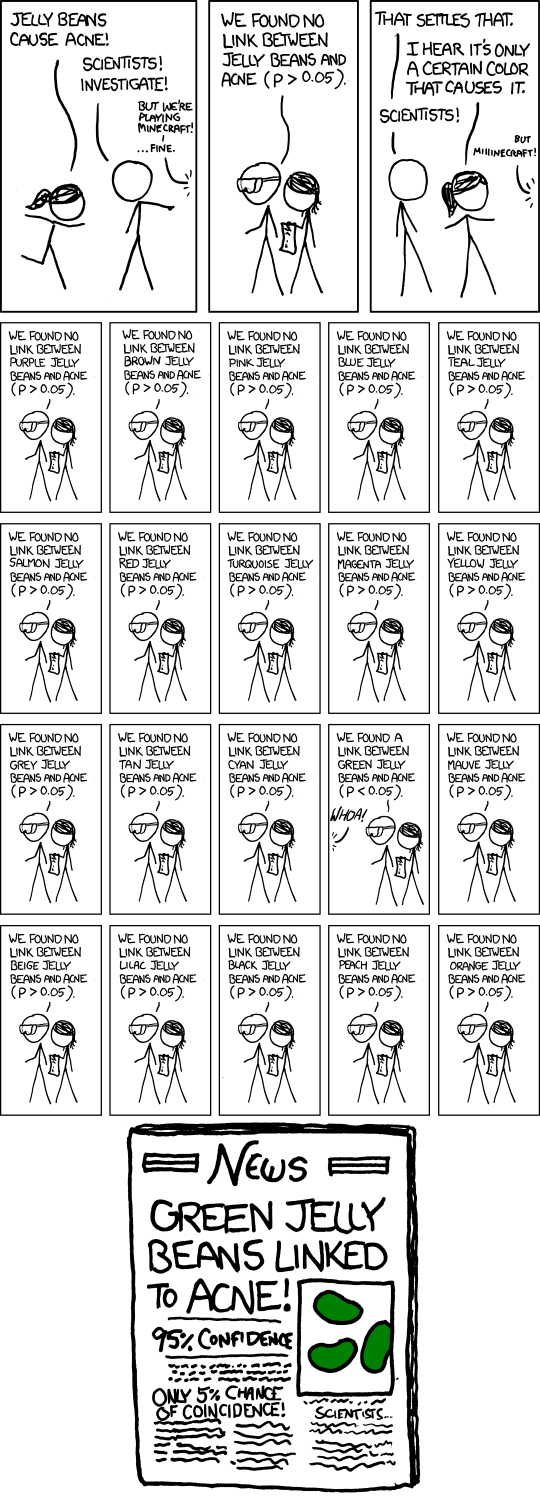
\includegraphics[width=0.3\textwidth]{images/significant.png}
\end{center}

\end{changemargin}
\end{frame}

\begin{frame}
\frametitle{Choice of Test}
\begin{changemargin}{1cm}

There are a number of tests from
which one could choose. 

The main thing to note here is the
prerequisites each tests requires for it to be sound.

For example, a number of tests require that the underlying
population is distributed normally.

\end{changemargin}
\end{frame}

\begin{frame}
\frametitle{Student's t-test}
\begin{changemargin}{1cm}

The requirements for the Student's t-test are: 
\begin{enumerate}
	\item the data is continuous, 
	\item the data follows a normal probability distribution
	\item the samples are independent, and
	\item they are simple random samples from the respective populations.
\end{enumerate}
\end{changemargin}
\end{frame}

\begin{frame}
\frametitle{Student's t-test}
\begin{changemargin}{1cm}

(1) is true if we assume that any value for time may
occur.

We ensure (3) and (4) from the manner in which we choose the samples. 

We satisfied (2) by assumption.
\end{changemargin}
\end{frame}

\begin{frame}
\frametitle{Results}
\begin{changemargin}{1cm}
Adding 250,000 integers starting from the empty set.

\begin{center}
    \begin{tabular}{l|c|c}
	\textbf{Implementation} & \textbf{Average} & \textbf{Std.~Dev.}\\ \hline
	\texttt{HashSet} & $0.183095$ & $0.00124$ \\ \hline
	\texttt{LinkedHashSet} & $0.20011$ & $0.000609$ \\ \hline
	\texttt{TreeSet} & $0.3975$ & $0.00222$ \\
    \end{tabular}
\end{center}

\end{changemargin}
\end{frame}

\begin{frame}
\frametitle{Results}
\begin{changemargin}{1cm}
Querying each of the 250,000 integers that have been added.

Our queries are elements we know to be in the set only.

\begin{center}
    \begin{tabular}{l|c|c}
	
	\textbf{Implementation} & \textbf{Average} & \textbf{Std.~Dev.}\\ \hline
	\texttt{HashSet} & $0.029934$ & $0.000685$ \\ \hline
	\texttt{LinkedHashSet} & $0.083366$ & $0.001148$ \\ \hline
	\texttt{TreeSet} & $0.097701$ & $0.002612$ \\
    \end{tabular}
\end{center}

\end{changemargin}
\end{frame}

\begin{frame}
\frametitle{Hypothesis Tests}
\begin{changemargin}{1cm}

We now articulate null hypothesis,
and a choice for the threshold $p$ value, and conduct our tests.

we have chosen a two-tailed, unpaired
Student's t-test. 

Again, we urge you to take a stats course
to understand the test in more depth.

\end{changemargin}
\end{frame}

\begin{frame}
\frametitle{Hypothesis Tests}
\begin{changemargin}{1cm}

As $p$ value, we choose, say, $0.01$, i.e., $1\%$. 

This choice
is arbitrary, and really depends on what your peers will accept.

In conducting a hypothesis test in the context of the discovery
of Higgs Boson, for example, the $p$ value was chosen as
``five-sigma'' (i.e., $5$ times the standard deviation), which
corresponds to a $p$ threshold value of $3\times 10^{-7}$.

We choose a much more conservative threshold of $0.01$.
So, we reject the null hypothesis if the calculated probability
is less than $0.01$.


\end{changemargin}
\end{frame}

\begin{frame}
\frametitle{Hypothesis Tests}
\begin{changemargin}{1cm}

The Student's t-test run with our above mean, standard deviation
and $N$ (number of samples, which in our case is $30$) produces
the following output:
\begin{quote}
    The two-tailed P value is less than $0.0001$.
\end{quote}

That is, the computed probability is less than our threshold
probability of $0.01$.

 Therefore, we reject the null hypothesis!

\end{changemargin}
\end{frame}

\begin{frame}
\frametitle{Our Alternate Hypothesis}
\begin{changemargin}{1cm}

Our alternate hypothesis is that there
is a difference in performance. 

But not that a particular one
of those is better than the other. 

However, we could informally
look at our data and conclude that our experiments suggest that
\texttt{HashSet} performs better than \texttt{LinkedHashSet}, given all our
assumptions and choices.

\end{changemargin}
\end{frame}

\begin{frame}
\frametitle{}
\begin{changemargin}{1cm}


\end{changemargin}
\end{frame}

\begin{frame}
\frametitle{The Other Comparisons}
\begin{changemargin}{1cm}

We can similarly perform the other two comparisons,
\texttt{HashSet} vs. \texttt{TreeSet}, and \texttt{LinkedHashSet}
 vs. \texttt{TreeSet}, and get
similar results.

Similarly, a Student's t-test for the
null hypothesis, ``there is no difference in querying 250,000
members of \texttt{LinkedHashSet} and \texttt{TreeSet}'' using our data from
the table above for querying produces the same output as above:
\begin{quote}
    The two-tailed P value is less than $0.0001$.
\end{quote}

\end{changemargin}
\end{frame}


\begin{frame}
\frametitle{Multiple Compaisons}
\begin{changemargin}{1cm}

Are we done? Unfortunately, not quite. 

We have performed a pairwise comparison of three groups. 

This is an example of a situation that makes
us susceptible to a problem known as \emph{multiple comparisons}.

The problem is that we posed multiple hypotheses using the same
data.

Therefore, the chance that we see statistical significance
in some pairwise comparison is increased purely by chance.

\end{changemargin}
\end{frame}


\begin{frame}
\frametitle{Multiple Comparisons}
\begin{changemargin}{1cm}

We have a probability of
$0.01$ of erroneously rejecting each null hypothesis if indeed
the null hypothesis is true. 

We have, however, posed three
such hypotheses.

Therefore,
$\text{Pr}\{\ge 1 \text{ erroneous rejection}\} =
1 - \text{Pr}\{\text{no erroneous rejection}\} =
1 - (0.99)^3 \approx 0.03 > 0.01$. 

\end{changemargin}
\end{frame}

\begin{frame}
\frametitle{Addressing the Multiple Comparisons Problem}
\begin{changemargin}{1cm}
Our strategy is the Bonferroni Correction.

To test
$k$ hypotheses with a desired significance level of
$s$, we test each hypothesis at a significance level
of $s/k$. 

In our case, $k=3$, and so we need to test
each of our pairwise hypotheses at a threshold of
$0.0033$ so that the family of tests has a threshold
of $0.01$.


\end{changemargin}
\end{frame}


\begin{frame}
\frametitle{Bonferroni Correction}
\begin{changemargin}{1cm}

In our case, the computed probability
based on the data is less than $0.0033$ for each test,
so our conclusions are remain valid.

The Bonferroni correction is conservative, i.e.,
overkill, and therefore safe. 

A more exact
correction can be applied instead.

Details omitted from this lecture.

\end{changemargin}
\end{frame}


\begin{frame}
\frametitle{Closing}
\begin{changemargin}{1cm}

This is just an introduction to the use of statistics in evaluating
software performance.

The techniques are sound but this is a complicated
subject and the brief overview in this lecture is by no means a substitute
for a full course on statistics.

It should serve to alert you to the issues.

\end{changemargin}
\end{frame}



\end{document}
